\section{Empirical Results}\label{sec:experiment}

In this section we present the empirical results obtained from running Hash-join, LIP and LIP-$k$ on several datasets. In Section \ref{sec:dataset}, we present the datasets we use and describe how we generate skewed and adversarial datasets. In Section \ref{sec:time} we present the running time of multiple strategies and discuss their performance. In Section \ref{sec:ratio} we discuss how $k$ affects the competitive ratio of LIP-$k$ empirically on our datasets.

\subsection{Datasets}
\label{sec:dataset}


\subsubsection{Skew Datasets}

We modify the normal \texttt{LINEORDER} file produced by the SSB data generator with SF = 1 to produce the four skewed \texttt{LINEORDER} tables listed below.
For simplicity in generating skew tables, we skew the \texttt{ORDER DATE} foreign key in the \texttt{LINEORDER} table, corresponding to the primary key of the \texttt{DATE} table. 
We alter the distribution of \texttt{ORDER DATE} foreign keys satisfying \texttt{DATE.YEAR = 1997 OR DATE.YEAR = 1998}, which we will shorten to \texttt{SKEW PRED}.
Let 

\begin{itemize}
    \item \texttt{LINEORDER-DATE-FIRST-HALF}: Let $N$ be the total number of batches in \texttt{LINEORDER}. 
    The first $N/2$ batches have $\sigma_{\texttt{SKEW PRED}} = 1$ while the remaining $N/2$ batches have $\sigma_{\texttt{SKEW PRED}} = 0$.
    In other words, The first $N/2$ batches contain only keys satisfying \texttt{SKEW PRED}, 
    while the next $N/2$ batches contain only keys not satisying \texttt{SKEW PRED}, 
    and so on. 

    \item \texttt{LINEORDER-DATE-50-50}: The first 50 batches have $\sigma_{\texttt{SKEW PRED}} = 1$ while the next 50 batches have $\sigma_{\texttt{SKEW PRED}} = 0$, and so on.

    \item \texttt{LINEORDER-DATE-LINEAR}: $\sigma_{\texttt{SKEW PRED}}$ increases linearly from 0 to 1 across the \texttt{LINEORDER} table, 
    {\it i.e.} batch $k$ has $\sigma_{\texttt{SKEW PRED}} = k/N$.

    \item \texttt{LINEORDER-DATE-PART-ADVERSARY}: We defer discussion on this dataset to Section~\ref{sec:ratio}, 
    as it requires a careful description of its construction.

\end{itemize} 






Skewed datasets are generated by first generating the SSB dataset with $\text{SF} = 1$.
We then edit the columns we want to skew. 



We summarize the skew datasets studied in this paper in Table~\ref{tab:skew_datasets}

\begin{center}
\begin{tabular}{ |>{\ttfamily}l|>{\ttfamily}c|l| } 
\hline
{\bf Dataset Name} & {\bf Skewed Foreign Keys} & {\bf Description of Skew} \\
\hline
\hline
LINEORDER-UNIFORM& N/A & No skew. Generated from SSB data generator.\\
\hline
LINEORDER-DATE-FIRST-HALF& ORDER DATE & $\sigma_{\texttt{SKEW PRED}}$ changes from 1 to 0 halfway through\\
& &  the table.\\
\hline
LINEORDER-DATE-50-50& ORDER DATE & $\sigma_{\texttt{SKEW PRED}}$ changes from 1 to 0 or from 0 to 1 \\
& & every 50 batches. \\ 
\hline
LINEORDER-DATE-LINEAR& ORDER DATE & $\sigma_{\texttt{SKEW PRED}}$ increases linearly from 0 to 1 \\
& & through the table. \\
\hline
LINEORDER-DATE-PART-ADVERSARY& ORDER DATE & See Section~\ref{sec:ratio}\\
& PART KEY & \\
\hline
\end{tabular}
\end{center}

The adversarial dataset is constructed to make SSB query 4.2 achieve near worst-case performance for LIP. 


\subsection{Execution Time}
\label{sec:time}



SSB query groups 1 and 2 do not join on \texttt{ORDER DATE} and are thus unaffected by the skewed key column. 
Fig.~\ref{fig:times0} shows execution times for these queries on the \texttt{LINEORDER-DATE-50-50}.
As expected, we observe that LIP and LIP-$k$ have roughly equal performance for these queries.
Henceforth, we will exclude query groups 1 and 2 from our analysis, 
as they provide us no insight. 
Nevertheless, from these results, we can conclude that the extra overhead associated with LIP-$k$ is negligible.



However, query groups 3 and 4 -- except for query 4.1 -- do join on \texttt{ORDER DATE}, so our skew can potentially affect the execution of LIP and LIP-$k$ on these queries.
We include only queries from groups 3 and 4 in our analysis. 
Query 4.1 is included as well as a "sanity check"; LIP and LIP-$k$ should have roughly equal performance on this query.

Fig.~\ref{fig:times1}(a) shows execution times using \texttt{LINEORDER-DATE-FIRST-HALF}. 
We see that LIP and LIP-$k$ have roughly equal performance on queries 3.2, 3.3, 3.4, and 4.3 (in addition to 4.1).
In such queries, we do not gain much by responding to local changes in the key distribution,
since one of the \texttt{SUPPLIER} filter is already very selective. 
LIP applies the \texttt{SUPPLIER} filter first.
In brief, it is "good enough" to apply a very selective filter first, even if it is not optimal.
On the other hand, LIP-$k$ performs better on queries 3.1 and 4.2, 
since the other filters are not particularly selective. 
We also observe that smaller $k$ has slightly better performance, 
because small $k$ can respond much more quickly to the sudden change in selectivity.

Fig.~\ref{fig:times1}(b) shows execution times using \texttt{LINEORDER-DATE-50-50}. 

The key observation is that LIP-$k$ must first "miss" before it can respond to a sudden change in selectivity.
For example, consider LIP-1 processing the $101^{st}$ batch in \texttt{LINEORDER-DATE-50-50}. 
At this point, the \text{DATE} filter has selectivity 0, and is thus probed first. 
However, the \texttt{DATE} filter eliminates no tuples in the current batch, since the current batch has selectivity 1.
Hence, LIP-1 performs an entire batch of unnecessary probes. 
Afterwards, LIP-1 then knows to push the \texttt{DATE} filter to end of the filter sequence. 
In general, every time the batch selectivity switches from 0 to 1, 
LIP-1 performs an entire batch of unnecessary probes. 

Because these queries already have a very selective \texttt{SUPPLIER} filter, 

The cost associated with responsiveness may outweigh its benefit. 

Fig.~\ref{fig:times2}(a) shows execution times using \texttt{LINEORDER-DATE-LINEAR}. 
The key difference between this dataset and the others is that the skew is smooth. 
We observe that LIP-$k$ performs worse than LIP on queries 3.3 and 4.3. 
The argument we applied to explain L

\begin{figure}
    \centering
    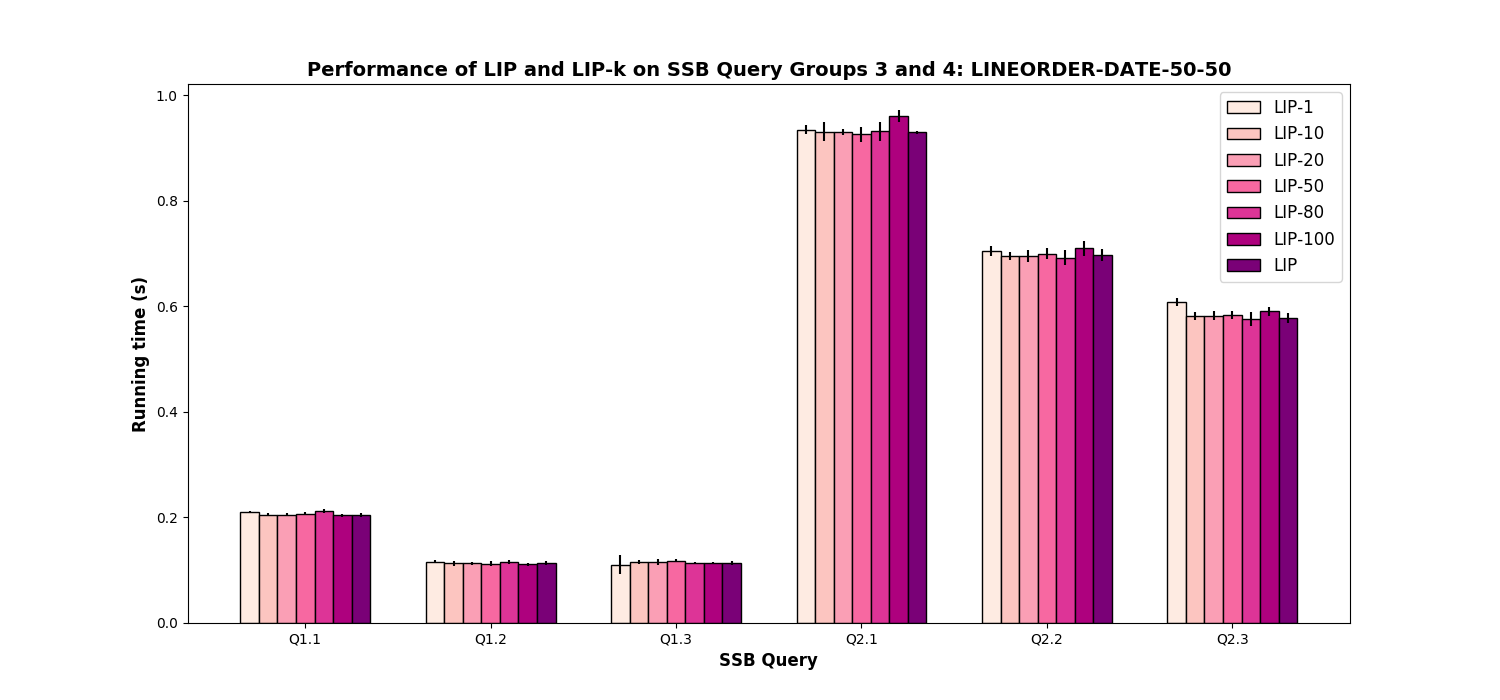
\includegraphics[width=0.9\textwidth,keepaspectratio]{lip-and-lipk-date-50-50-q1-q2}
    \caption{Execution time for SSB query groups 1 and 2 on \texttt{LINEORDER-DATE-50-50}}
    \label{fig:times0}
\end{figure}

\begin{figure}
    \centering
    \subfloat[]{
        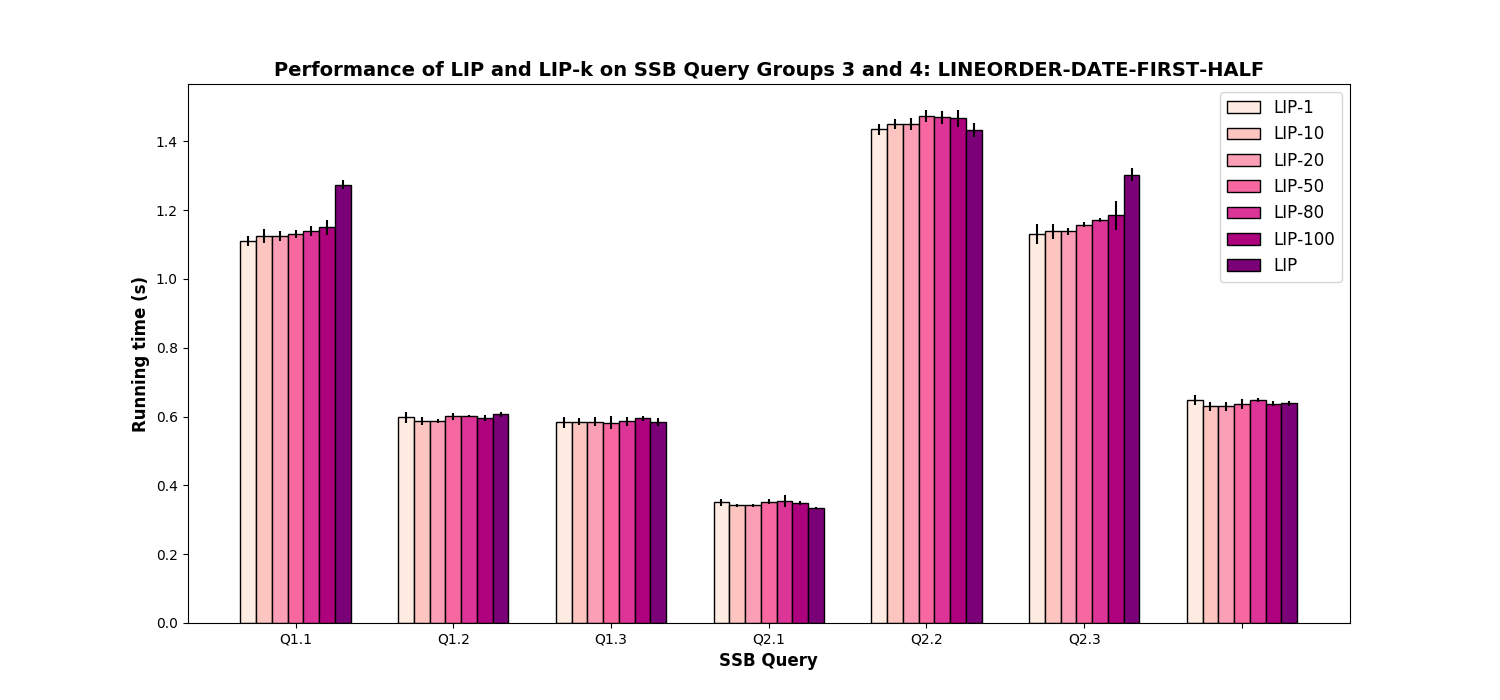
\includegraphics[width=0.9\textwidth,keepaspectratio]{lip-and-lipk-date-first-half}
    }\\
    \subfloat[]{
        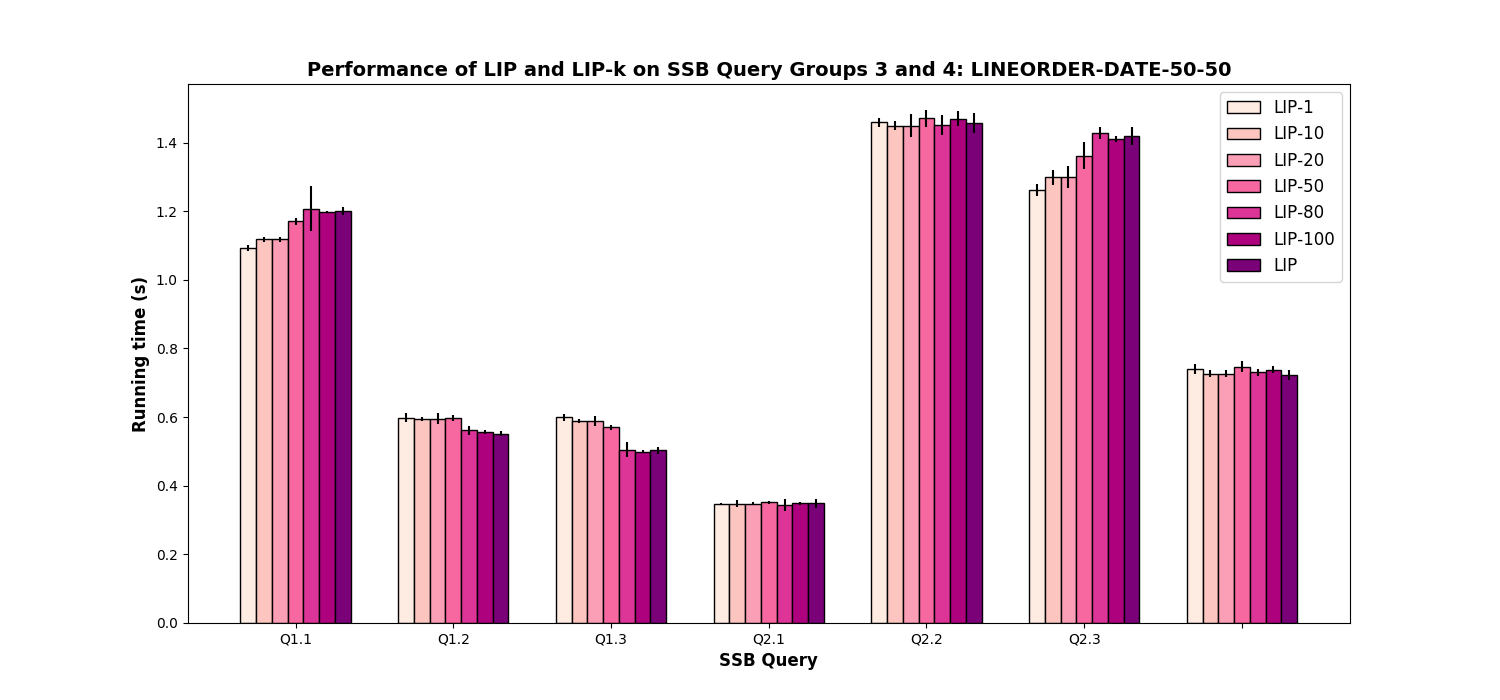
\includegraphics[width=0.9\textwidth,keepaspectratio]{lip-and-lipk-date-50-50}
    }
    \caption{Execution time for SSB query groups 3 and 4 on (a) \texttt{LINEORDER-DATE-FIRST-HALF} and (b)~\texttt{LINEORDER-DATE-50-50}}
    \label{fig:times1}
\end{figure}


\begin{figure}
    \centering    
    \subfloat[]{
        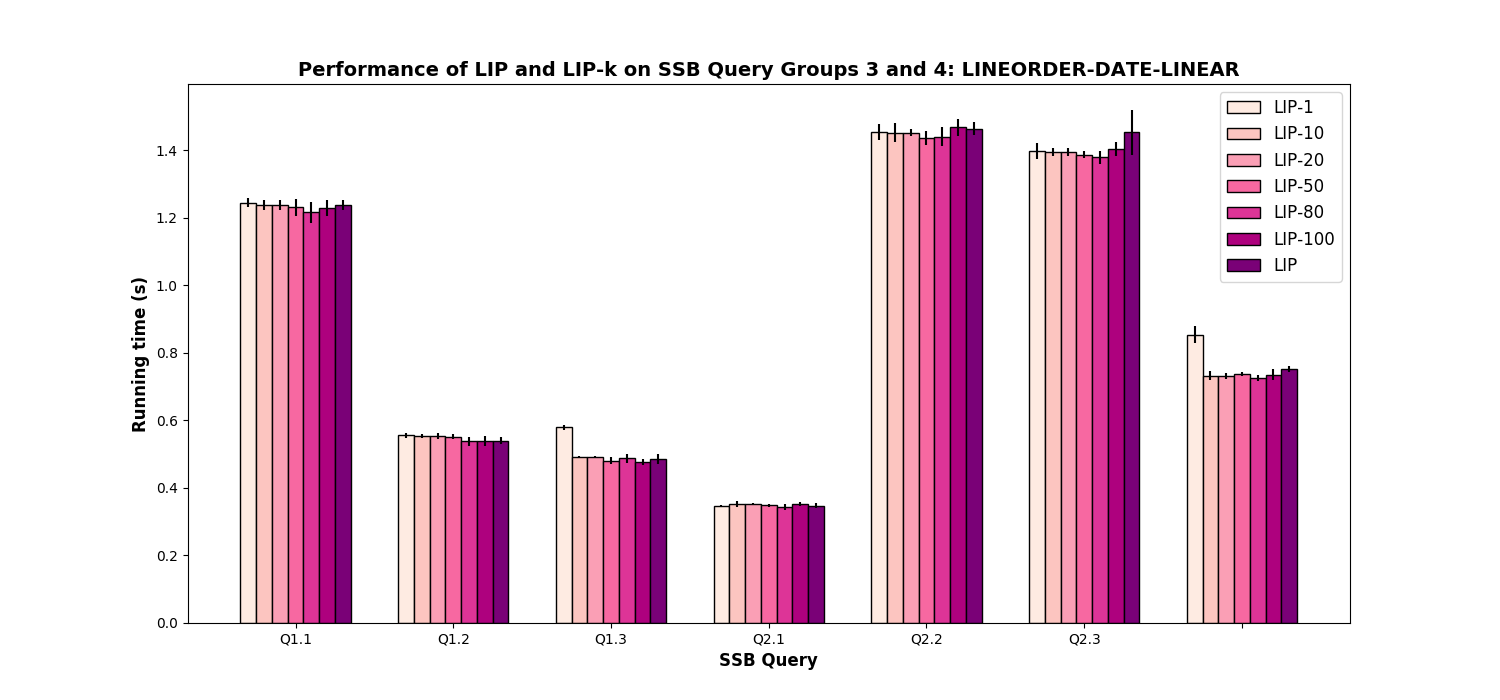
\includegraphics[width=0.9\textwidth,keepaspectratio]{lip-and-lipk-date-linear}
    }\\
    \subfloat[]{
        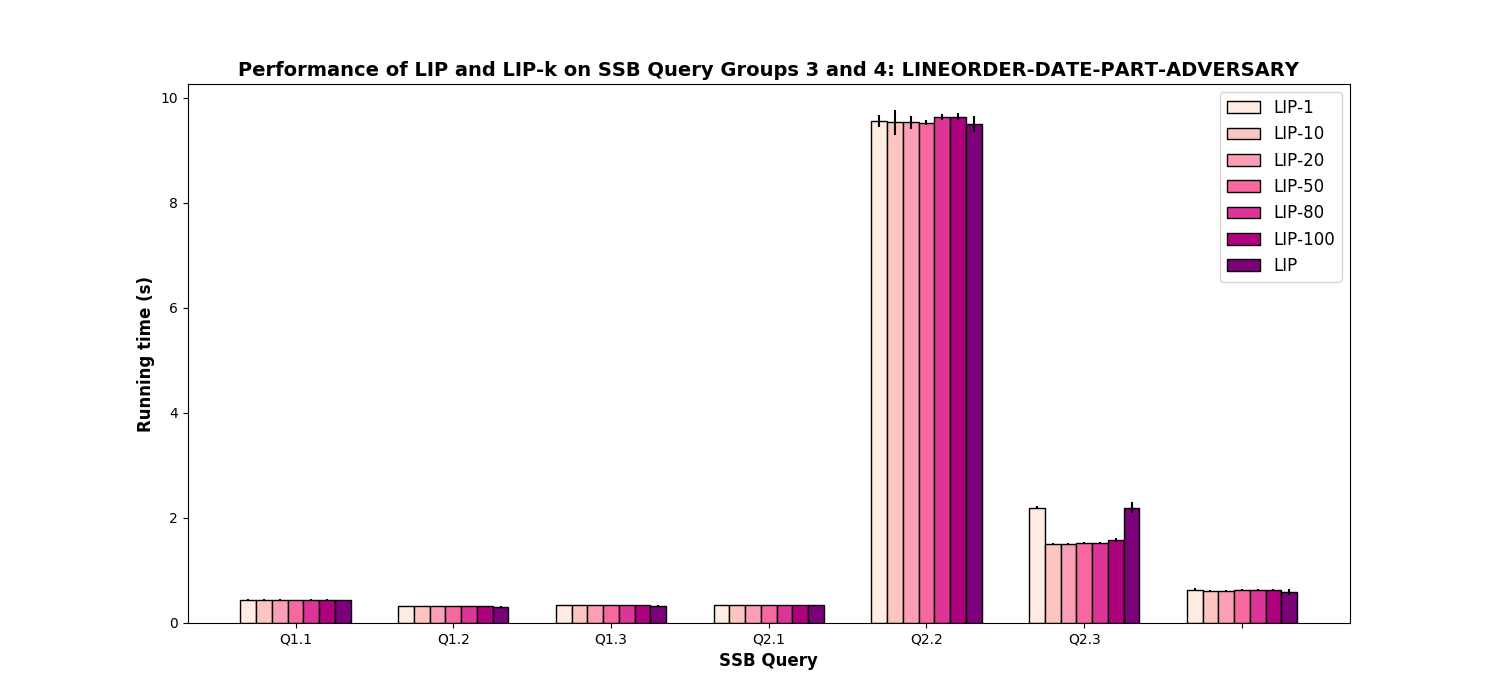
\includegraphics[width=0.9\textwidth,keepaspectratio]{lip-and-lipk-date-part-adversary}
    }
    \caption{Execution time for SSB query groups 3 and 4 on (a) \texttt{LINEORDER-DATE-LINEAR} and (b)~\texttt{LINEORDER-DATE-PART-ADVERSARY}}
    \label{fig:times2}
\end{figure}



\subsection{Competitive Ratio}
\label{sec:ratio}

To empirically support \ref{thm:det-n}, we construct an adversarial dataset which forces LIP to perform the maximum number of filter probes possible.
We now show how to generally construct such a dataset where $n = 2$, mimicking the proof of Theorem \ref{thm:det-n}.

Suppose we are joining our fact table with two dimension tables A and B using LIP.
Let $f_i^A$ denote the selectivity of the Bloom filter for A after processing the $i^{th}$ batch. 
Let $\sigma_i^A$ denote the selectivity of the Bloom filter for A on the $i^{th}$ batch alone. 
Define analogous quantities for dimension table B.

We start with the first fact table batch having
$\sigma_1^A = \frac{1}{2} - \varepsilon$ and $\sigma_1^B = \frac{1}{2} + \varepsilon$ where $0 < \varepsilon < \frac{1}{2}$. Then for all $j > 1$, we let

\begin{equation*}
\sigma_j^A = 
    \begin{cases}
    1 & \text{if $j$ is even} \\[0.5em]
    0 & \text{if $j$ is odd} \\
    \end{cases} \quad \text{and }
\sigma_j^B = 
    \begin{cases}
    0 & \text{if $j$ is even} \\[0.5em]
    1 &  \text{if $j$ is odd} \\
    \end{cases}
\end{equation*}

Thus, the optimal filter sequence $S^{OPT}$ for $j > 1$ is 

\begin{align*}
S^{OPT} &= 
    \begin{cases}
    (B, A) & \text{if $j$ is even} \\[0.5em]
    (A, B) & \text{if $j$ is odd} \\
    \end{cases}\\[0.5em]
\end{align*}

\DeclarePairedDelimiter\floor{\lfloor}{\rfloor}
After processing batch $j > 1$, we have 
$f_j^A = \frac{\frac{1}{2} - \varepsilon + \floor{\frac{j}{2}}}{j}$ 
and 
$f_j^B = \frac{\frac{1}{2} + \varepsilon + \floor{\frac{j}{2}}}{j}$  
which can be rewritten as

\begin{equation*}
f_j^A = 
    \begin{cases}
    \frac{1}{2} + \frac{\frac{1}{2}-\varepsilon}{j} & \text{if $j$ is even} \\[0.5em]
    \frac{1}{2} - \frac{\varepsilon}{j} &  \text{if $j$ is odd} \\
    \end{cases}  \quad \text{and }
f_j^B = 
    \begin{cases}
    \frac{1}{2} - \frac{\frac{1}{2}-\varepsilon}{j} & \text{if $j$ is even} \\[0.5em]
    \frac{1}{2} + \frac{\varepsilon}{j} &  \text{if $j$ is odd} \\
    \end{cases}\\[0.5em]
\end{equation*}

Since $\frac{1}{2} - \varepsilon > 0$, LIP's filter ordering for $j > 1$ will be

\begin{align*}
S &= 
    \begin{cases}
    (A, B) & \text{if $j$ is even} \\[0.5em]
    (B, A) & \text{if $j$ is odd} \\
    \end{cases}\\[0.5em]
\end{align*}

which is the reverse of $S^{OPT}$. 
Hence, after the first batch has been processed, LIP will have worst-case performance on all remaining batches. 
As the number of batches in the fact table increases, the competitve ratio of LIP on such a dataset approaches $n =2$.

Following this construction, we generated an adversarial dataset for SSB query 4.2 with A = \texttt{DATE} and B = \texttt{PART},
excluding the joins on the \texttt{CUSTOMER} and \texttt{SUPPLIER} dimension tables.
\footnote{In reality, we do not exclude the joins on \texttt{CUSTOMER} and \texttt{SUPPLIER} in query 4.2. 
Rather, we generate the adversarial dataset such that $\sigma_i^{\texttt{CUSTOMER}}=1$ and $\sigma_i^{\texttt{SUPPLIER}}=1$ for every batch $i$. 
This achieves the same effect as excluding the joins, though. 
This was done because it is much easier to generate an adversarial dataset on fewer dimension tables.}



We ran LIP and LIP-$k$ on the uniform dataset and each skewed dataset computed the competitive ratio of each algorithm by taking the maximum of the competitive ratios achieved across all queries in all datasets. In fact, the dataset responsible for the greatest competitive ratio for all algorithms is the adversarial dataset.  The results are depicted in Figure \ref{fig:cr}. 

\begin{figure}
    \centering
    \subfloat[]{
        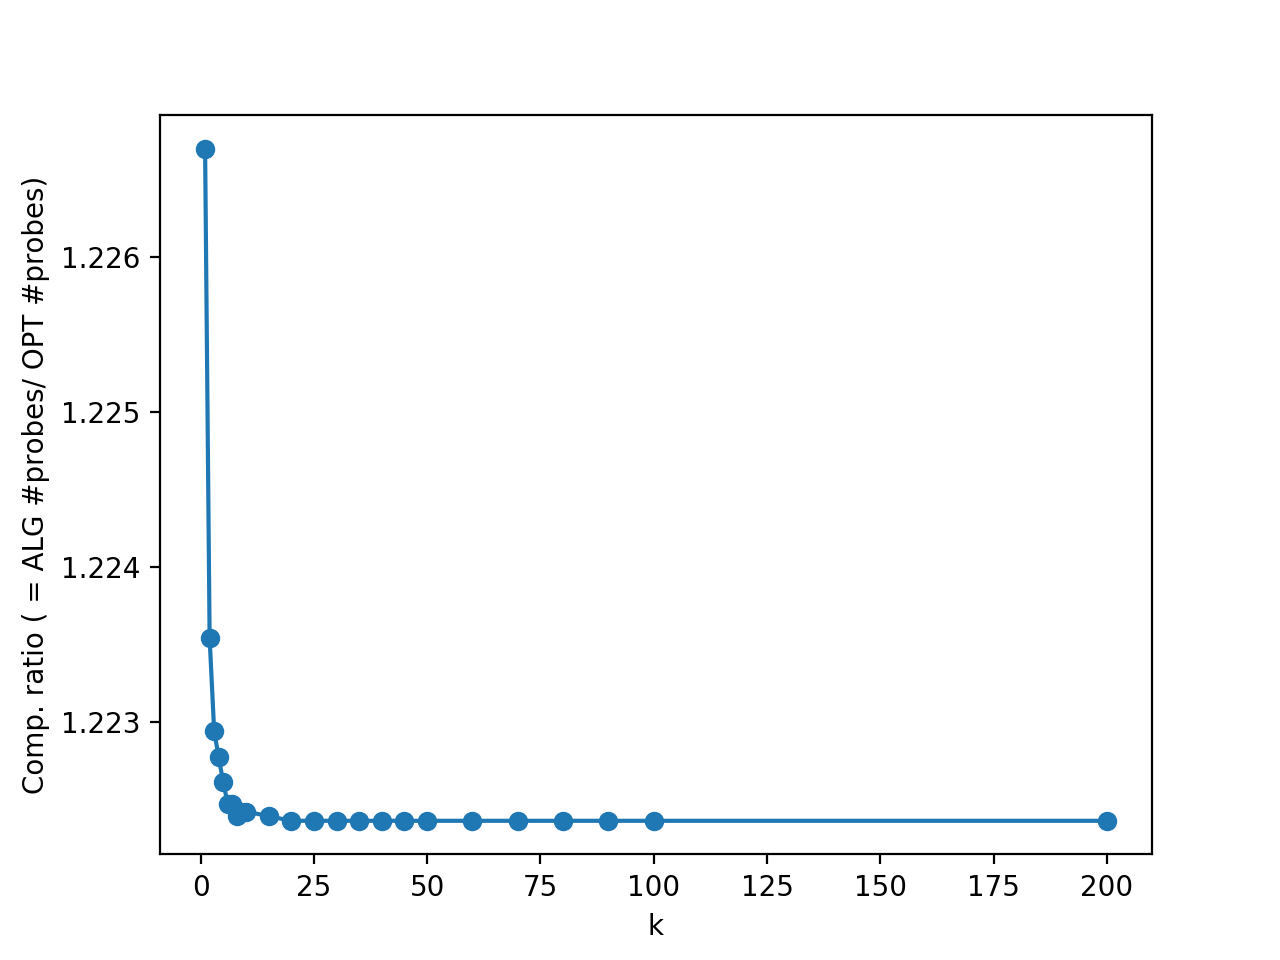
\includegraphics[width=0.43\textwidth,keepaspectratio]{cr-k-uniform}
    }   
    \quad
    \subfloat[]{
        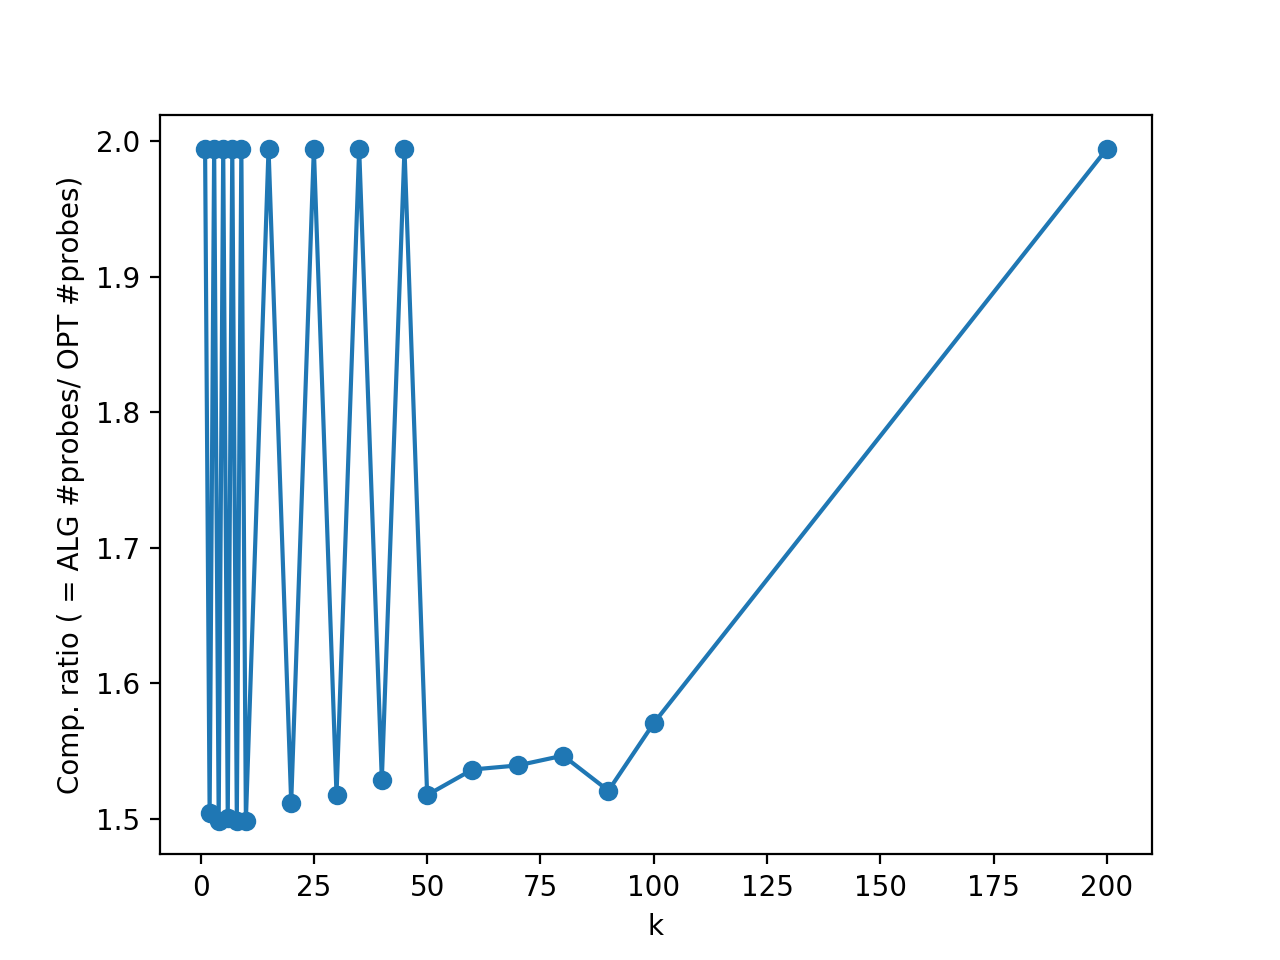
\includegraphics[height=0.32\textwidth,keepaspectratio]{cr-k-skewed}
    }
    \caption{The competitive ratios of LIP-$k$ against different $k$ values. We ran LIP-$k$ on uniform data and skewed (and adversarial) dataset to produce (a) and (b) respectively. The data point at $k = 200$ represents LIP (which is essentially LIP-$\infty$).}
    \label{fig:cr}
\end{figure}

When the keys in the fact table columns are distributed uniformly, the filters need not react to the local changes. Hence for LIP with higher $k$, it remembers more batches in the uniform data, therefore may produce a more accurate estimate of the selectivities than the LIP-$k$ with smaller $k$. Hence, the competitive ratio decreases slightly as $k$ increases, as depicted in Figure \ref{fig:cr}.

%@TODO: Explain the adversarial case using epsilons
Figure \ref{fig:cr}(b) displays how an adversarial dataset can make LIP-$k$ and LIP perform poorly. Each LIP-$k$ with even $k$ achieves an approximation ratio less than 2; LIP and LIP-$k$ with odd $k$ achieve an approximation ratio of almost 2 precisely at Query 3.2 in dataset \texttt{date-part-adversary}. Query 3.2 has two joins, and thus the performance of LIP-$k$ with even $k$ matches the worst case competitive ratio. By construction of \texttt{date-part-adversary}, the first batch has $\sigma^{1}_{1} = 1/2-\
\varepsilon$ and $\sigma^{1}_{2} = 1/2+\varepsilon$, and  each batch $B_{2i+1}$ is an \textit{odd} batch, with $\sigma^{2i}_{1} = 0$ and $\sigma^{2i}_{2} = 1$; and each batch $B_{2i}$ is an \textit{even} batch, with $\sigma^{2i}_{1} = 1$ and $\sigma^{2i}_{2} = 0$. 

When $i \leq k$, LIP and LIP-$k$ execute identically, since LIP-$k$ has not yet ``forgotten" any previous batches. We now consider the case where $i > k$, {\it i.e.} where LIP-$k$ has forgotten at least the first batch. For odd $k$, LIP-$k$'s selectivity estimates always contains one more odd (or even) batch than the other, and thus the estimated selectivity and filtering sequence are in favor of the majority batch type. This yields a false prediction of the next batch, yielding a competitive ratio of 2. For even $k$, LIP-$k$'s selectivity estimates contain an equal amount of even an odd batches,  and thus estimated selectivities remain the same ($1/2$ by construction) throughout the execution, and the filter sequence does not change. Thus for at most half of the batches it is optimal, and for the other half it is worse, resulting in a competitive ratio of at least \[ \frac{1 \times 1/2 + 2 \times 1/2}{1} = 1.5,\] as depicted in Figure \ref{fig:cr}. For LIP, since it remembers the statistics from the beginning, by construction it would also make the same decision as LIP-$k$ with odd $k$, losing at every batch. 

LIP performs poorly because it never forgets the first batch.
%@TODO: I will explain this better!!!!
\footnote{An astute observer might notice that for $k = 200$, the worst-case competitive ratio of $2$ is achieved even though $k$ is not odd. This is explained by recognizing that LIP-200 is essentially an approximation of LIP. LIP-200 performs just as poorly as LIP up until  the $201^{st}$ batch, after which it estimates both selectivities as 1/2.}



\begin{align*}
\varepsilon_i = 
    \begin{cases}
    \frac{\varepsilon}{2k+1} & \text{for odd $i$, where $i = 2k + 1$} \\ 
    \frac{\frac{1}{2} - \varepsilon}{2k} & \text{for even $i$, where $i = 2k$}
    \end{cases}
\end{align*}

If $k$ is even, then LIP-k will (after the first $k$ batches have been processed) have $\sigma^A_i = \sigma^B_i = \frac{1}{2}$. Thus,


%$k = 1, 2, 3, 4, 5, 10, 15, 20, 25, 30, 35, 40, 45, 50, 60, 70, 80, 90, 100$ on 